\documentclass[xcolor=dvipsnames]{beamer}
\usepackage{times}
\usepackage{graphicx,ulem,booktabs}
\usepackage{hhline}
\usepackage{transparent}
\usepackage{setspace}
\usepackage{xcolor}
\usepackage{dcolumn, multirow, transparent}
\usepackage{adjustbox} 
%\usepackage{avant} % PSNFSS Font, in every TeX distribution 
%\renewcommand{\familydefault}{\sfdefault}
%\usepackage{kpfonts} 
\usepackage{fbb}
\beamertemplatenavigationsymbolsempty
\setbeamertemplate{footline}[frame number]
\usepackage[english]{isodate}
\setbeamercovered{transparent}
\setbeamercolor{section in toc}{fg=Fuchsia}

\newcommand{\textgb}[1]{\textcolor{OliveGreen}{\textbf{#1}}}
\newcommand{\textvb}[1]{\textcolor{Fuchsia}{\textbf{#1}}}
\newcommand{\textlb}[1]{\textcolor{LimeGreen}{\textbf{#1}}}
\newcommand{\texttb}[1]{\textcolor{Thistle}{\textbf{#1}}}

\mode<presentation>
{ \usetheme{boxes}\usecolortheme[named=OliveGreen]{structure}
\setbeamertemplate{blocks}[rounded][shadow=false]
\setbeamertemplate{itemize item}[default]
\setbeamertemplate{enumerate item}[default]
\setbeamercovered{invisible}
 \useinnertheme{} 
}

%\addtobeamertemplate{navigation symbols}{}{%
 %   \usebeamerfont{footline}%
  %  \usebeamercolor[fg]{footline}%
    %\hspace{1em}%
   %  \usebeamerfont{author in foot}\insertshortauthor
    %\hspace{1em}\insertshortauthor\hfill%
    %\insertframenumber/\inserttotalframenumber
%}

\addtobeamertemplate{navigation symbols}{}{%
    \usebeamerfont{footline}%
    \usebeamercolor[fg]{footline}%
    \hspace{1em}%
    \insertframenumber/\inserttotalframenumber
}

% \color{OliveGreen}
% \color{LimeGreen}
% \color{Thistle}
% \color{Fuchsia}
% \color{RoyalPurple}


\title{\LARGE Title} 
\subtitle{Subtitile}
\author{Elena Pro}
\institute{\small European Institute \\ LSE}
\date{\small \printdayoff\today}

\begin{document}
\begin{frame}
\maketitle
\begin{figure}
    \centering
    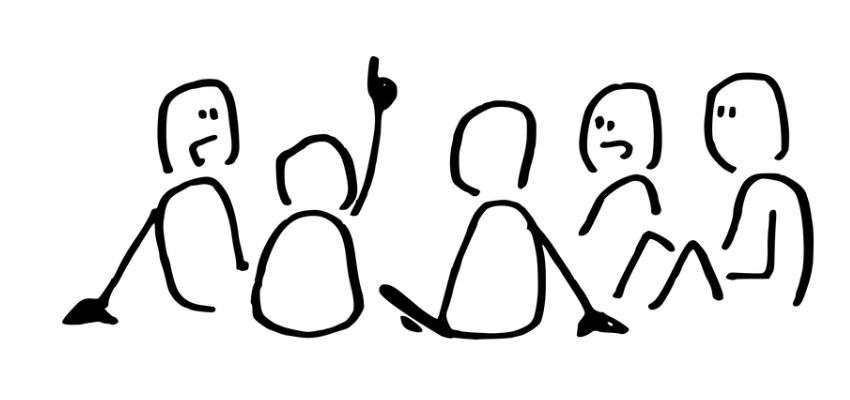
\includegraphics[width=0.5\linewidth]{Screenshot 2024-03-19 at 15.57.46.png}  
\end{figure}

\end{frame}

\begin{frame}
\frametitle{Table of Contents}
\tableofcontents
\end{frame}

\section{1. Context}
\begin{frame}{\color{OliveGreen} When I Becomes We}
List:
\begin{itemize}
    \item item 1
    \pause
    \item item 2
    \pause
    \item item 3
\end{itemize}
\end{frame}

\section{ 2. Theoretical Framework}
\begin{frame}{Where are we?}
\tableofcontents[currentsection, currentsubsection]   
\end{frame}
\begin{frame}{Title}
List:
\begin{enumerate}
    \item item 1
    \item \textvb{item 2}
    \begin{itemize}
        \item \textgb{item 2.1}
        \item \textlb{item 2.2}
        \item \texttb{item 2.3}
    \end{itemize}
    \item item 3
\end{enumerate}
\end{frame}


    \begin{frame}    
        \begin{itemize}[<+-| alert@+>]
            \setbeamercolor{alerted text}{fg=Fuchsia} %change the font color
            \setbeamerfont{alerted text}{series=\bfseries} %make alerted text bold
            \item Hello World
            \item Hello Earth
            \item Hello Sun
        \end{itemize}
        \uncover<+>{} %make the list all change to unbolded
    \end{frame}


\section{ 3. Methodology}

\begin{frame}{Where are we?}
\tableofcontents[currentsection, currentsubsection]   
\end{frame}

\begin{frame}{Methodology}
    
\end{frame}



    
\end{document}

    
